\documentclass[
 preprint,
 preprintnumbers,
 amsmath,amssymb,
 aps,
 pre,
 longbibliography,
 10pt, twocolumn
]{revtex4-1}

\usepackage{graphicx}% Include figure files
\graphicspath{{./figures/}} % path to figures
\usepackage{dcolumn}% Align table columns on decimal point
\usepackage{bm}% bold math
\usepackage{hyperref}% add hypertext capabilities
\usepackage{physics} % package for physics symbols


\begin{document}
% define commands
\newcommand{\eqnname}{Eqn.}
\newcommand{\secname}{Sec.}


\title{Rectification of energy and motion in active gyroscopic networks}

%\author{Zhenghan Liao, William Irvine, Suriyanarayanan Vaikuntanathan}
%\affiliation{Department of Chemistry and Physics and The James Franck Institute, University of Chicago, Chicago, IL, 60637}


\begin{abstract}
[Will be revised in the end] We study a model that combines gyroscopic networks and active matter. From numerical calculations, theory, and simulations, we show that autonomous heat flows are generated at the nonequilibrium steady state. Distinct from conventional heat flows that are driven by temperature difference at the boundaries, this heat flow is an emergent collective behavior. 
We then focus on understanding three issues: the mechanism of this nonzero heat flow, the connection between the flow in active system and that in the well-studied isolated system, and the relationship between the network geometry and the flow pattern. 
Understanding the last issue in turn enables us to control the flow pattern by the design of the network geometry.
\end{abstract}


\maketitle

%\tableofcontents


\section{Introduction} \label{sec:intro}
One of the longstanding problems in non-equilibrium statistical mechanics concerns uncovering principles for the rectification of energy and motion in many body microscopic systems. Success will enable molecular motors [{\bf this line has to change!}]. In this paper, we report on one attempt at construction of such design principles. Our central idea is to combine properties of mechanical networks, topology, and non-equilibrium activity. The resultant microscopic system rectifies energy and in some settings also motion. [{\bf This introductory paragraph will change and be expanded, this is a very very rough first pass}]. 

Designs of mechanical metamaterials have achieved unconventional mechanical properties or functions in a wide range of systems \cite{Bertoldi2017FlexibleMetamaterials}. Examples include negative Poisson ratios in auxetic metamaterials \cite{Lakes2017Negative-Poissons-RatioSolids,Ren2018AuxeticReview}, topological zero modes in isostatic lattices \cite{Kane2013TopologicalLattices,Lubensky2015PhononsLattices,Paulose2015SelectiveMetamaterials.}, unidirectional edge modes in topological gyroscopic metamaterials \cite{Nash2015TopologicalMetamaterials,Wang2015TopologicalWaves,Mitchell2018AmorphousSets}, and the allosteric effect in mechanical networks \cite{Rocks2017DesigningNetworks.,Yan2017ArchitectureMaterials.,Flechsig2017DesignProteins}. 


Gyroscopic metamaterials have been demonstrated to support peculiar topological edge modes, where the energy circulates along the network boundary unidirectionally \cite{Nash2015TopologicalMetamaterials}. These chiral energy circulations indicates some kind of Time-Reversal Symmetry (TRS) breaking. As a comparison, conventional normal modes do not break TRS, because the underlying Newton's equation is symmetric under time-reversal. Ref. \cite{Nash2015TopologicalMetamaterials} explained their TRS using an analogy between the gyroscopic equation and the Schrodinger equation, and showed that their TRS is related to the network geometry. The network does not break TRS when all its bonds are horizontal or vertical (e.g. a square network), and breaks TRS otherwise.
On top of this TRS-breaking, topological properties can be given through designed network structures, such as honeycomb-like structures \cite{Nash2015TopologicalMetamaterials} or more generally structures constructed from random point sets with some rules \cite{Mitchell2018AmorphousSets}. 

%In our work, we require the TRS-breaking part, but do not pay special attention to topological properties, so our discussion will be based on generic network structures.%energy flows in the combination of gyroscopic networks and non-equilibrium activity

%with less focus on the exotic mechanical modes and more on statistical properties.


In contrast to the increasing studies on mechanical properties, one less explored topic is the effect of thermal fluctuations. This effect is usually irrelevant, because the energy scale of the metamaterials is much larger than that of thermal fluctuations. However, fluctuations are inevitable if the system is made in micro-scale \cite{Blees2015GrapheneKirigami}. 
Indeed, some recent works have found an interesting interplay between thermal \cite{Rocklin2018FoldingTemperature,Pedro2018TopologicalInteractions} or nonequilibium \cite{Woodhouse2018AutonomousEquilibrium} fluctuations and the zero mode, which show promises in studying the effect of fluctuations.
In a similar spirit, we explore the correlations and rectified currents generated in the mechanical gyroscopic networks when in contact with a heat bath. 


When introducing fluctuations, a natural choice may be adding thermal fluctuations. However, this addition restores TRS, thus destroy the interesting energy flow. The reason is that, the gyroscopic network can be mapped to a spring-mass network with Lorentz force on the masses \cite{Lee2018TopologicalLaws}, and according to the Bohr-van Leeuwen theorem \cite{Pradhan2010NonexistenceSurface}, the steady-state distribution of such system is Boltzmann. Since the velocity term in Boltzmann distribution is quadratic, TRS is restored.

A next choice of fluctuations is nonequilibrium fluctuations, or active baths.
The active bath we use is the active Ornstein-Uhlenbeck particle (AOUP) model \cite{Fodor2016HowMatter}, which consists of a constant friction and an Ornstein-Uhlenbeck (OU) noise. The AOUP model has experienced a growing interest in recent years, because of its theoretical simplicity and its ability to capture many nonequilibrium and active matter phenomena.
To exemplify one class of studies, it was experimentally found that, colloids in a bacteria bath can be well-modeled by the AOUP model \cite{Wu2000ParticleBath}; this finding helps realizing the previously proposed thermal ratchet \cite{Magnasco1993ForcedRatchets} in the experiment \cite{Koumakis2013TargetedBacteria}, where the combination of bacteria bath and asymmetric barriers leads to targeted transport of colloids.

In the combined system of gyroscopic networks and active baths, we found averaged energy flows among sites{\bf explain since this is the first time you are using this phrase}. This energy flow is distinct from conventional ones which are driven by temperature differences. It utilizes the chiral modes in isolated gyroscopic networks, but it also has its own statistical properties.

The rest sections are organized as follows:
First, in \secname~\ref{sec:model} we introduce the network model. 
Then in \secname~\ref{sec:flux} we define the observable we focus on, the energy flux, and show numerical results that the active gyroscopic network can rectify energy flux.
\secname~\ref{sec:linear_response}-\ref{sec:path} are the main sections, which present theories of the flux. 
\secname~\ref{sec:linear_response} uses linear response theory to express the flux in terms of the response function, and arrive at \eqnname~\eqref{eqn:flux_integral} and \eqref{eqn:flux_residue}. These two equations contain all information we need for the flux, however, this information is not apparent because the equations are compact. In the next three sections, we rewrite the equations from different perspectives to give a comprehensive view on the energy flux.
\secname~\ref{sec:fourier} analyzes a generalization of \eqnname~\eqref{eqn:flux_integral}, and explains why there exists nonzero energy rectifications.
\secname~\ref{sec:eigenmode} rewrites \eqnname~\eqref{eqn:flux_residue} as a weighted sum over the eigenmodes of a reference system, which builds a connection between our model and previous studies on gyroscopic networks \cite{Nash2015TopologicalMetamaterials,Mitchell2018AmorphousSets}.
\secname~\ref{sec:path} decomposes \eqnname~\eqref{eqn:flux_residue} as a path summation, and since the shortest paths contribute the most, the sum can be approximated by only a few paths. Furthermore, this path analysis reveal how the flux depends on the network geometry.
\secname~\ref{sec:simulation}-\ref{sec:swimmer} are complementary to main theories. 
\secname~\ref{sec:simulation} shows the shape of energy flux as a function of time in a sample simulated trajectory.
\secname~\ref{sec:swimmer} discusses further implications of the rectification in a different context of swimming at low Reynolds numbers.
Finally, \secname~\ref{sec:conclusion} concludes the paper.

{\bf rewrite to focus more broadly on rectification, with the energy flow being one example and the potential motion being another. }


\section{Model} \label{sec:model}

\begin{figure}[ht]
	\centering
	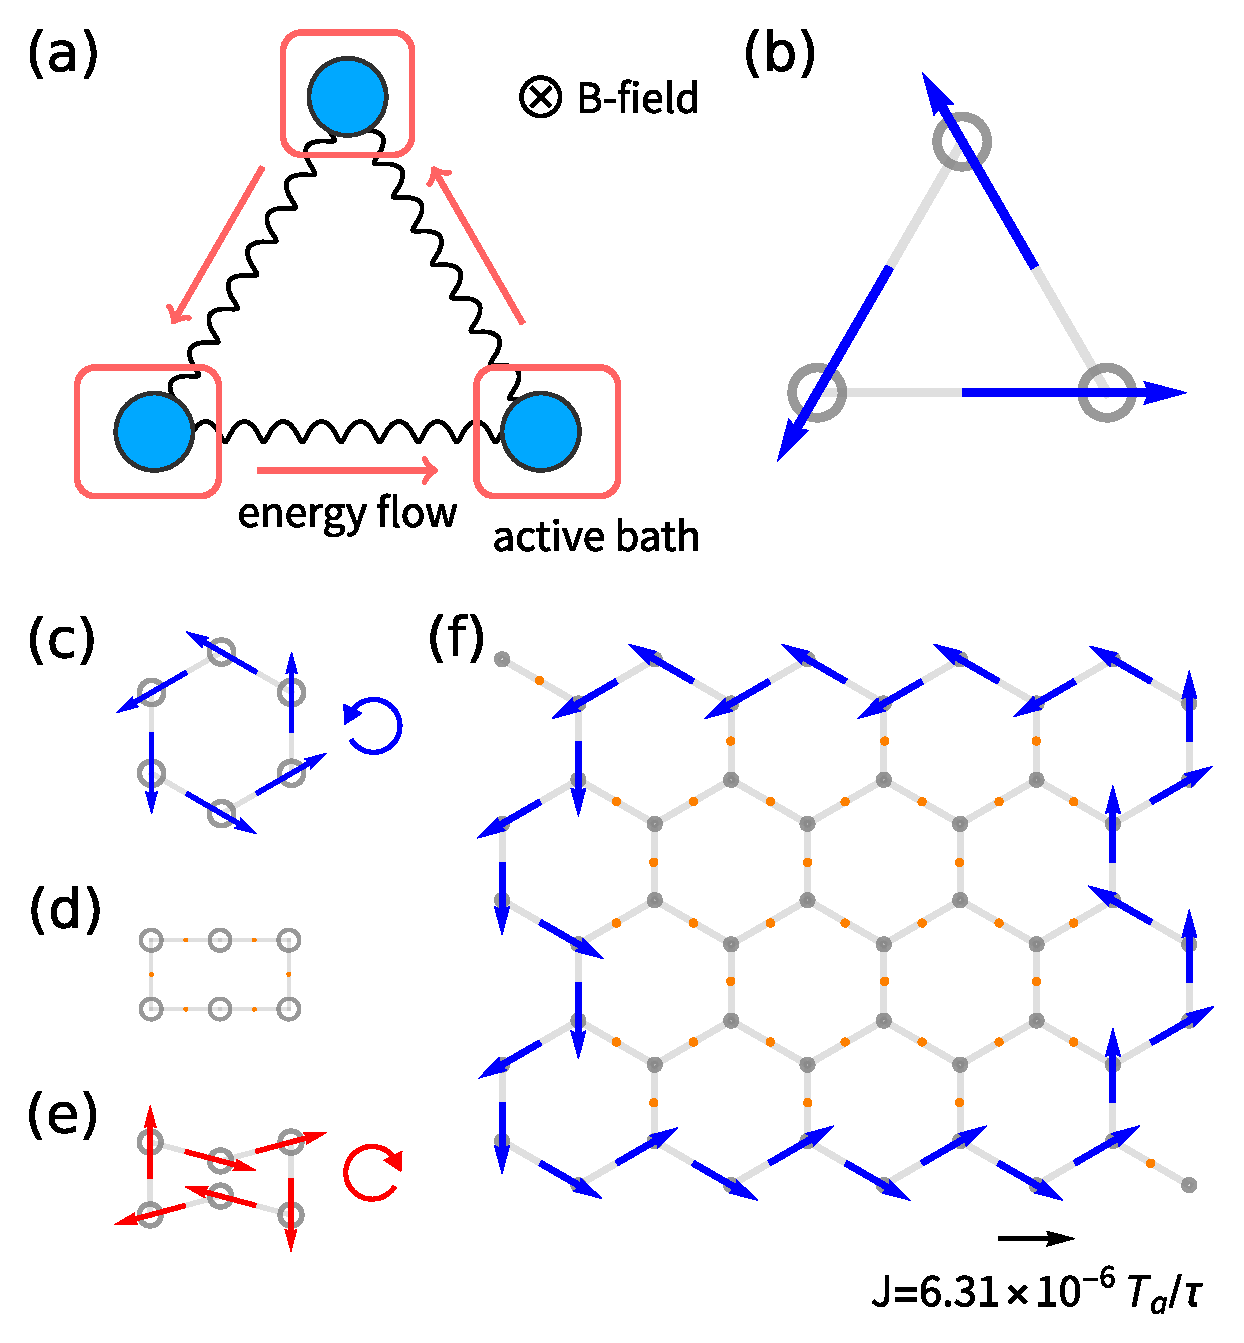
\includegraphics[width=0.45\textwidth]{1_model_and_result.pdf}
    \caption{The model and the heat flux in polygonal and more complex networks. All parameters are set to $1$. 
    (a) Schematic of the model. It is a spring-mass network with Lorentz force and active bath on each mass. 
    (b-f) Heat flux results from numerical calculations. Gray circles and lines represent the network geometry. Arrows represent the direction and magnitude of the heat flux. Fluxes are colored blue if it is counter-clockwise (CCW), red if clockwise (CW), and orange otherwise. For complex networks, fluxes smaller than $1/10$ of the scale bar are not shown for clarity. 
    (b) Triangle network has CCW heat flux, $\expval{J}=1.61\times 10^{-3} T_a/\tau$.  
    (c-e) In hexagon networks, the flux direction changes with the geometry. Flux magnitude in both (c),(e) is $6.26\times 10^{-6} T_a/\tau$. 
    (f) The flux pattern in the honeycomb network shows localization on the boundary and CCW direction.
    }
    \label{fig:model_and_result}
\end{figure}

Our model (\figurename~\ref{fig:model_and_result}) uses spring-mass network with Lorentz force instead of gyroscopic networks, because the former is more convenient, and it does not lose relevant properties of the latter \cite{Lee2018TopologicalLaws}.
The equation of motion reads
\begin{equation} \label{eqn:GLE_single}
m\dot{\bm{v}}_i = -k_g \bm{z}_i + \sum_j\bm{F}_{ji} + \bm{v}_i\times\bm{B} - \gamma\bm{v}_i + \bm{\eta}_i ,
\end{equation}
where $z_i \equiv \begin{pmatrix} x_i & y_i \end{pmatrix}^T$ is the displacement of particle $i$ from its mechanical equilibrium position.

The first three terms on the right-hand side describe a spring-mass network with Lorentz force. 
The first term is the on-site restoring force.
The second term is the spring force from the bonded neighbors $j$'s,
$F_{ji} = k (e_{ij}^T z_i + e_{ji}^T z_j) (-e_{ij})$.
Here the force is linearized by assuming the natural length of springs are much larger than the scale of particles' displacement, and $e_{ij}$ is the unit vector from the equilibrium position of $i$ to that of $j$.
The third term $\bm{v}_i\times\bm{B}$ is the Lorentz force (the electric charge is absorbed in $\bm{B}$), and we set $\bm{B} = -B\mathbf{\hat{z}}$. 
The on-site potential and the Lorentz force together gives the effect of a gyroscope.

The last two terms describe the active bath, which consists of friction $-\gamma v_i$ and OU colored noise $\eta_i$.
The colored noise has finite correlation time $\tau$ and strength $T_a$ ($T_a$ has the unit of energy)
\begin{equation} \label{eqn:noise_correlation}
\expval{\eta_i(t)\eta_{j}^T(t')} = I\delta_{i,j}\frac{\gamma T_a}{\tau} e^{-\frac{|t-t'|}{\tau}} ,
\end{equation}
where $I$ is the identity matrix with a proper dimension.
This OU noise can be conveniently modeled by a OU process \cite{Hanggi1994ColoredSystems}
\begin{equation} \label{eqn:noise_eom}
\tau \dot{\eta}_i = -\eta_i + \sqrt{2\gamma T_a}\xi_i ,
\end{equation}
where $\xi_i$ is the standard Gaussian white noise.
The friction and noise do not satisfy fluctuation-dissipation relation, thus driving the system out of equilibrium.
Only in the $\tau \rightarrow 0$ limit, the active bath reduces to the equilibrium Langevin bath.


\section{Energy flux definition and results{\bf Change title: if you want to be more descriptive, make it full sentences}} \label{sec:flux}
{\bf Maybe you can motivate here why we chose to look at energy flows. I am basically looking for a better opening paragraph for this section. This isn't a very specific request, I apologize, anything that makes the flow between this and the previous section better will be amazing}
There are two types of energy flows in the stochastic dynamics of the network: the energy exchange between particles and active baths, and the energy flow among particles.
Our focus is the second type, the time-averaged energy flux among particles at the steady state.

To arrive at a formula for this energy flux, first we define the energy of a particle as the sum of its kinetic energy, on-site potential energy, and one half of the bond energies \cite{Lepri2003ThermalLattices}, then using a stochastic version of derivation in \cite{Lepri2003ThermalLattices}, one gets (Supplemental Material)
\begin{equation} \label{eqn:flux_def}
\expval{J_{ij}} = \expval{\frac{1}{2} (\mathbf{v}_j \cdot \mathbf{F}_{ij} - \mathbf{v}_i \cdot \mathbf{F}_{ji})}
= \expval{\mathbf{v}_j \cdot \mathbf{F}_{ij}},
\end{equation}
where $\expval{J_{ij}}$ is the averaged energy flux from particle $i$ to $j$.
The second expression tells that this energy transfer equals the rate of microscopic work done on particle $j$ from $i$.
Since this microscopic work is due to particles' stochastic motions, rather than an external control, this energy flux is also a heat flux \cite{Sekimoto1998LangevinThermodynamics,Lepri2003ThermalLattices}.

To compute the value of heat flux $\expval{J}$, 
one needs to specify the system by the network geometry and parameters $m, k_g, k, B, \gamma, \tau, T_a$;
then from the linear equation of particles \eqnname~\eqref{eqn:GLE_single} and the colored noise \eqnname~\eqref{eqn:noise_eom}, one can numerically solve for the covariance between the displacement and the velocity using linear algebra \cite{Gardiner2009TheEquations,Ceriotti2010Colored-NoiseCarte};
finally, the flux \eqnname~\eqref{eqn:flux_def}, which is bilinear in displacement and velocity, can be extracted from the covariance.
(Supplemental Material)
Numerical calculations are performed using Mathematica \cite{WolframResearch2018Mathematica11.3} with custom code.

Main results are shown in \figurename~\ref{fig:model_and_result}. First, we see nonzero circulatory heat fluxes in the network (\figurename~\ref{fig:model_and_result}b). Second, the flux direction or pattern changes with the network geometry (\figurename~\ref{fig:model_and_result}c-f).

This heat flow is distinct from the conventional one driven by temperature differences, because in our system, the bath on all particles are identical. 
Unconventional heat flows have been studied in some other contexts, for example, heat radiation in a special equilibrium system with nonreciprocal magneto-optical nanoparticles \cite{Zhu2016PersistentTransfer}, baths that have nonuniform higher-order moments \cite{Kanazawa2013HeatFluctuations}, transverse heat flow in thermal Hall effect with cylindrical geometries \cite{Nomura2012Cross-correlatedSuperfluids,Zhang2016BerryEffects}, and thermal ratcheting using time-periodic protocols \cite{Li2008RatchetingBias,Ren2010EmergenceBias,Ren2012GeometricSystems}.
In our active gyroscopic network context, it is curious{\bf weird choice, say something other than curious} to ask how the heat flow is generated.

Specifically, we are interested in three main questions: what is the mechanism of this energy rectification, what is the connection between the flow in the active system and that in the well-studied isolated system, and what is the relationship between the network geometry and the flow pattern.

\section{Linear response theory for energy flux} \label{sec:linear_response}
{\bf I would suggest reorganizing this section so that you start with Eq 7 and then introduce the rest.}
To approach the above questions, in this section we use linear response theory to derive formulae \eqnname~\eqref{eqn:flux_integral} and \eqref{eqn:flux_residue} for the energy flux in this section, then in the next three sections interpret these equations from three perspectives, each targeted towards a different question.

Define the Fourier transform (FT) of a variable $f$ over a time period $t$ as $\tilde{f}(\omega) = \frac{1}{t} \int_0^t dt'\ f(t')e^{-i\omega t'}$, and represent the displacement of all particles by a column vector $z=\sum_i \ket{i}\otimes z_i$, with $\ket{i}$ denoting the 2D subspace of $i$,
then we get the FT of the equation of motion 
\begin{gather} \label{eqn:response}
    \tilde{z}(\omega) = G^+(\omega) \tilde{\eta}(\omega), \\
    G^{+}(\omega) \equiv [K + i\omega(\gamma I + BA) - m\omega^2I]^{-1},
\end{gather}
where $G^+$ is the response matrix, matrix $K$ calculates all on-site and spring forces $F$ by $F=-Kz$, and $A$ is an antisymmetric matrix $A=\sum_i \ket{i}\bra{i}\otimes \mqty(0 & 1 \\ -1 & 0)$.
This equation describes how the displacement $z$ responses to the noise $\tilde{\eta}$.

Following the procedure in \cite{Kundu2011LargeChains}, the flux defined in \eqnname~\eqref{eqn:flux_def} can be expressed using $G^+$ as a spectral integral (Supplemental Material)
\begin{equation} \label{eqn:flux_integral}
\expval{J} = \int_{-\infty}^\infty \dd{\omega} \frac{1}{1+\omega^2\tau^2} [-\frac{T_a k}{2\pi} \Re \tr G^+(\omega)A^{as}] ,
\end{equation}
where $A^{as}$ is an antisymmetric matrix
$A^{as} = -\ket{i}\bra{j} \otimes e_{ij}e_{ji}^T + \ket{j}\bra{i} \otimes e_{ji}e_{ij}^T$.
The response function $G^+(\omega)$ has no pole in the lower-half complex plane, but the colored noise introduces one pole at $\omega = -i/\tau$. Using the residue theorem we get (Supplemental Material)
\begin{equation} \label{eqn:flux_residue}
\frac{\expval{J}}{T_a/\tau} = -\frac{k}{2} \tr G^+(-\frac{i}{\tau})A^{as} .
\end{equation}
\eqnname~\eqref{eqn:flux_integral} and \eqref{eqn:flux_residue} serve as our starting point to understand the heat flux.

Before moving on, we note that the fluxes satisfy Kirchoff's law, i.e. on average there is no energy exchange between particles and the active bath. This can be shown by calculating the average heat exchange between particle $i$ and the active bath $\expval{\eta_i^T v_i - \gamma v_i^T v_i}$, which results in zero.
This Kirchoff's law puts a strong constraint on the flux among particles, and some corollaries immediately follow, such as networks with no cycles cannot have nonzero flux, and fluxes of all bonds in a polygon network (as in \figurename~\ref{fig:model_and_result}b-e) are equal.


\section{Ingredients for energy rectification and their roles{\bf Change title ! Say something descriptive: Decompposing the energy flux into modes etc etc that conveys the central purpose of the section}} \label{sec:fourier}

\begin{figure}[ht]
	\centering
	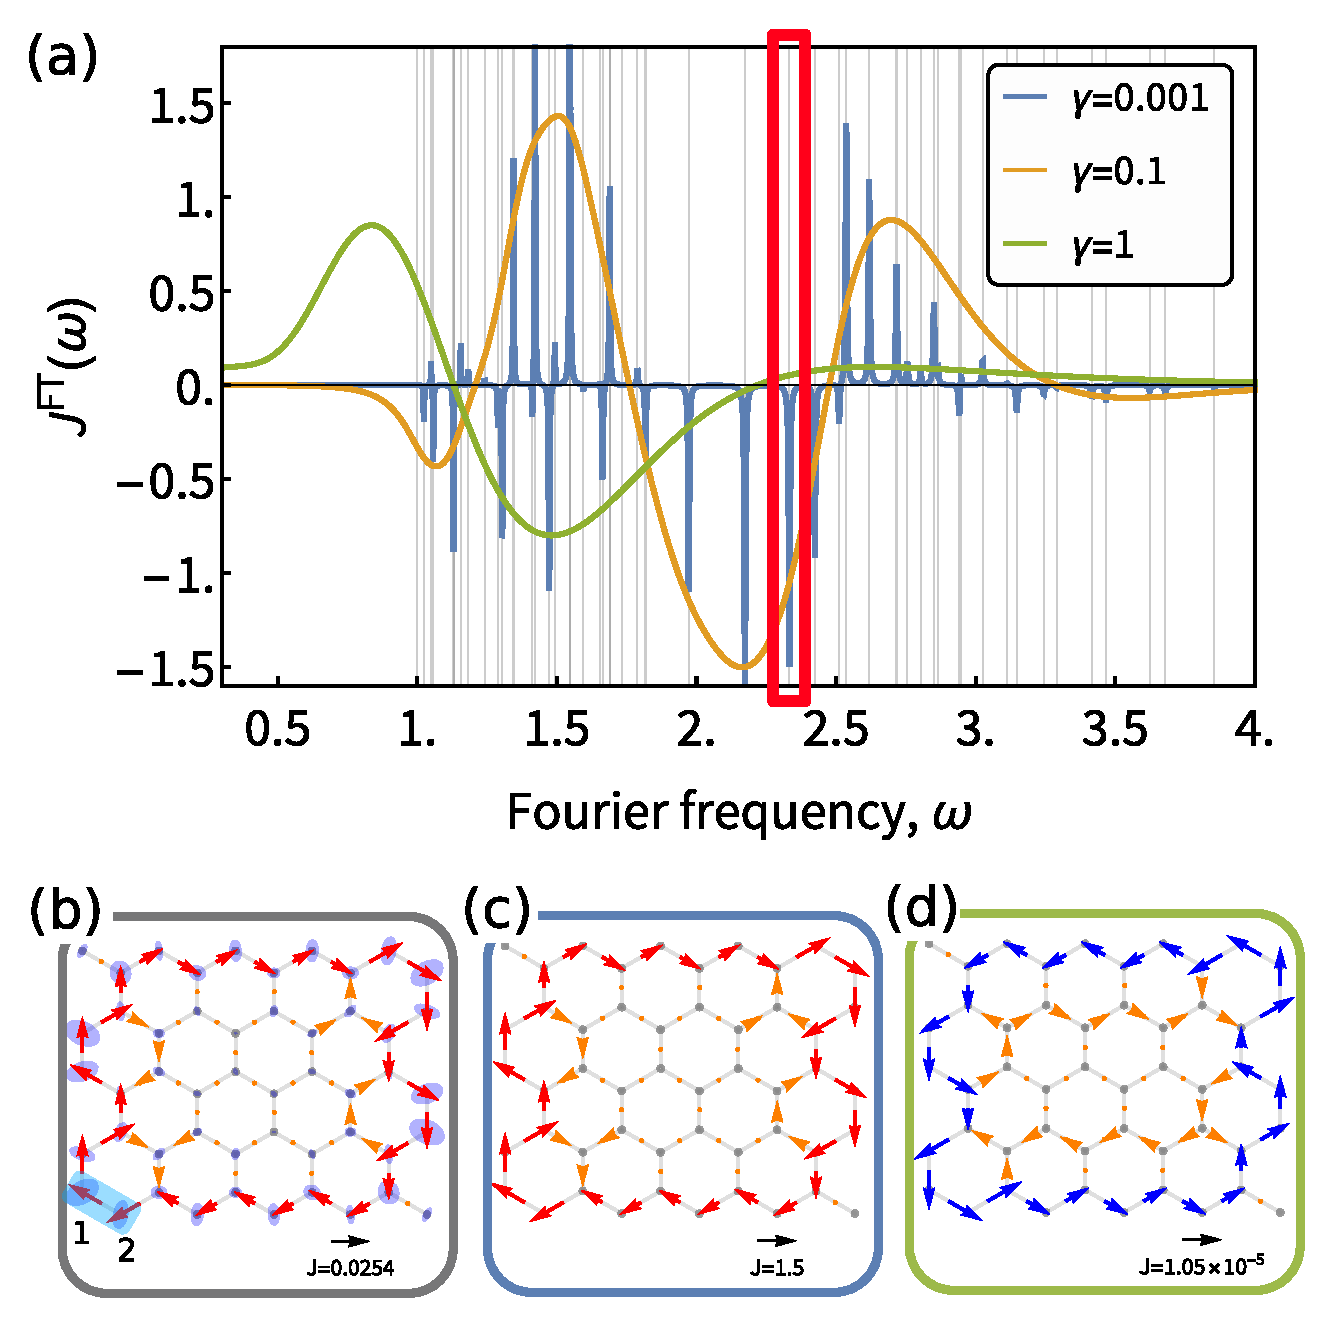
\includegraphics[width=0.45\textwidth]{2_Fourier_modes.pdf}
    \caption{The Fourier modes in the honeycomb network have nonzero fluxes, which at small $\gamma$'s originates from the chiral eigenmodes. For a better comparison between the Fourier mode and the eigenmodes studied in \cite{Nash2015TopologicalMetamaterials}, we use $1$st order dynamics (by setting $m=0$). All other parameters are set to $1$. 
    (a) Flux $J^{FT}(\omega)$ from particle $1$ to $2$ (highlighted in (b)) as a function of Fourier frequency $\omega$ for $\gamma=0.001,0.1,1$. For plotting purposes, $J^{FT}(\omega)$ for $\gamma=0.1,1$ are scaled up by $50,5000$, respectively. Positive (negative) $J^{FT}(\omega)$ corresponds to CCW (CW) flux. Gray vertical lines mark the frequency of eigenmodes. 
    (b-d) Comparison of the eigenmode and Fourier modes at frequency $2.33$.
    (b) The eigenmode is localized on the boundary. Blue disks represent the orbit of particles. 
    (c) The Fourier mode at small $\gamma$'s ($\gamma=0.001$) resembles the eigenmode.
    (e) The Fourier mode at larger $\gamma$'s ($\gamma=1$) is dissimilar to the eigenmode.
    }
    \label{fig:Fourier_modes}
\end{figure}

{\bf Maybe you can help the reader by providing a short summary of what the purpose of this section is... }
Compared with a simple thermal spring-mass network, the extra components in our model are the Lorentz force and the colored noise. Are they minimal ingredients for energy rectification, and what are their roles? 
By analyzing the integral \eqnname~\eqref{eqn:flux_integral}, we show that they are minimal ingredients, and each plays a different role.

To see this, we label two components of the integral as $\expval{J} = \int_{-\infty}^\infty \dd{\omega} h(\omega) J^{FT}(\omega)$, with $J^{FT}(\omega) \equiv -\frac{T_a k}{2\pi} \Re \tr G^+(\omega)A^{as}$ and $h(\omega)=\frac{1}{1+\omega^2\tau^2}$. 
$J^{FT}(\omega)$ is the flux at Fourier frequency $\omega$, which is a property of the damped isolated network, and is independent of the noise (apart from a constant $T_a$). 
$h(\omega)$ is the the noise spectrum (apart from a prefactor), $\expval{\tilde{\eta}(\omega)\tilde{\eta}^*(\omega)} = \frac{2\gamma T_a}{t}h(\omega)$. 

To generate a nonzero flux, first $J^{FT}(\omega)$ should not be zero everywhere {\bf awkward sentence, rewrite}. 
This is indeed the case as shown in \figurename~\ref{fig:Fourier_modes}a. 
In the small $\gamma$ regime, $J^{FT}(\omega) \neq 0$ is easily known, because the slightly damped system resonates near the eigen-frequencies of the undamped system, and the response (\figurename~\ref{fig:Fourier_modes}c) resembles the eigenmode (\figurename~\ref{fig:Fourier_modes}b), which is known to have nonzero energy fluxes \cite{Nash2015TopologicalMetamaterials}. 
More generally, $J^{FT}(\omega) \neq 0$ is due to the nonreciprocity from the Lorentz force. If $B=0$, the response $G^+$ is symmetric or reciprocal, and since $A^{as}$ is antisymmetric, the trace $\tr G^+(\omega) A^{as}=0$ at all $\omega$'s. Nonzero $B$ breaks the reciprocity of $G^+$, thus the trace can be nonzero.

Nonzero $J^{FT}(\omega)$ alone does not ensure a nonzero total flux, one further requires $h(\omega)$ to be nonconstant.
If $h(\omega)$ is constant, it corresponds to a white noise, and the system would be in equilibrium. In this case, the integral is always zero regardless of the value of $J^{FT}(\omega)$, because the response function $G^+(\omega)$ has no pole in the lower-half plane due to causality, thus the flux as a contour integral vanishes.
The nonconstant noise spectrum is in line with the nonequipartition perspective of the active system \cite{Lee2017FluctuationSystems.}.

The $h(\omega)$ for OU noise is indeed nonconstant, and it puts more weight on small $\omega$'s.
In fact the OU noise is just one choice of the non-white noise, and any nonconstant noise spectrum $h(\omega)$ is likely to shift the integral away from zero.
However, $h(\omega)=\frac{1}{1+\omega^2\tau^2}$ is arguably the simplest nontrivial noise. Because it only has one pole in the lower-half complex plane, which makes the evaluation of the integral as easy as evaluating the integrand at only one point; in addition, $\tr G^+(\omega)A^{as}$ at this pole $\omega=-i/\tau$ is real, so one can skip the evaluation of the $Re$ part in $J^{FT}(\omega)$. As a result, the flux as an integral \eqnname~\eqref{eqn:flux_integral} can be reduced to a much simpler formula \eqnname~\eqref{eqn:flux_residue}.

We see that the mechanism for rectification is a weighted excitation of chiral Fourier modes, where chiral modes are induced by the $B$-field via breaking the reciprocity of response, and the weight is provided by non-white noises via breaking the energy equipartition.


\section{Connection to isolated gyroscopic networks} \label{sec:eigenmode}

\begin{figure}[ht]
	\centering
	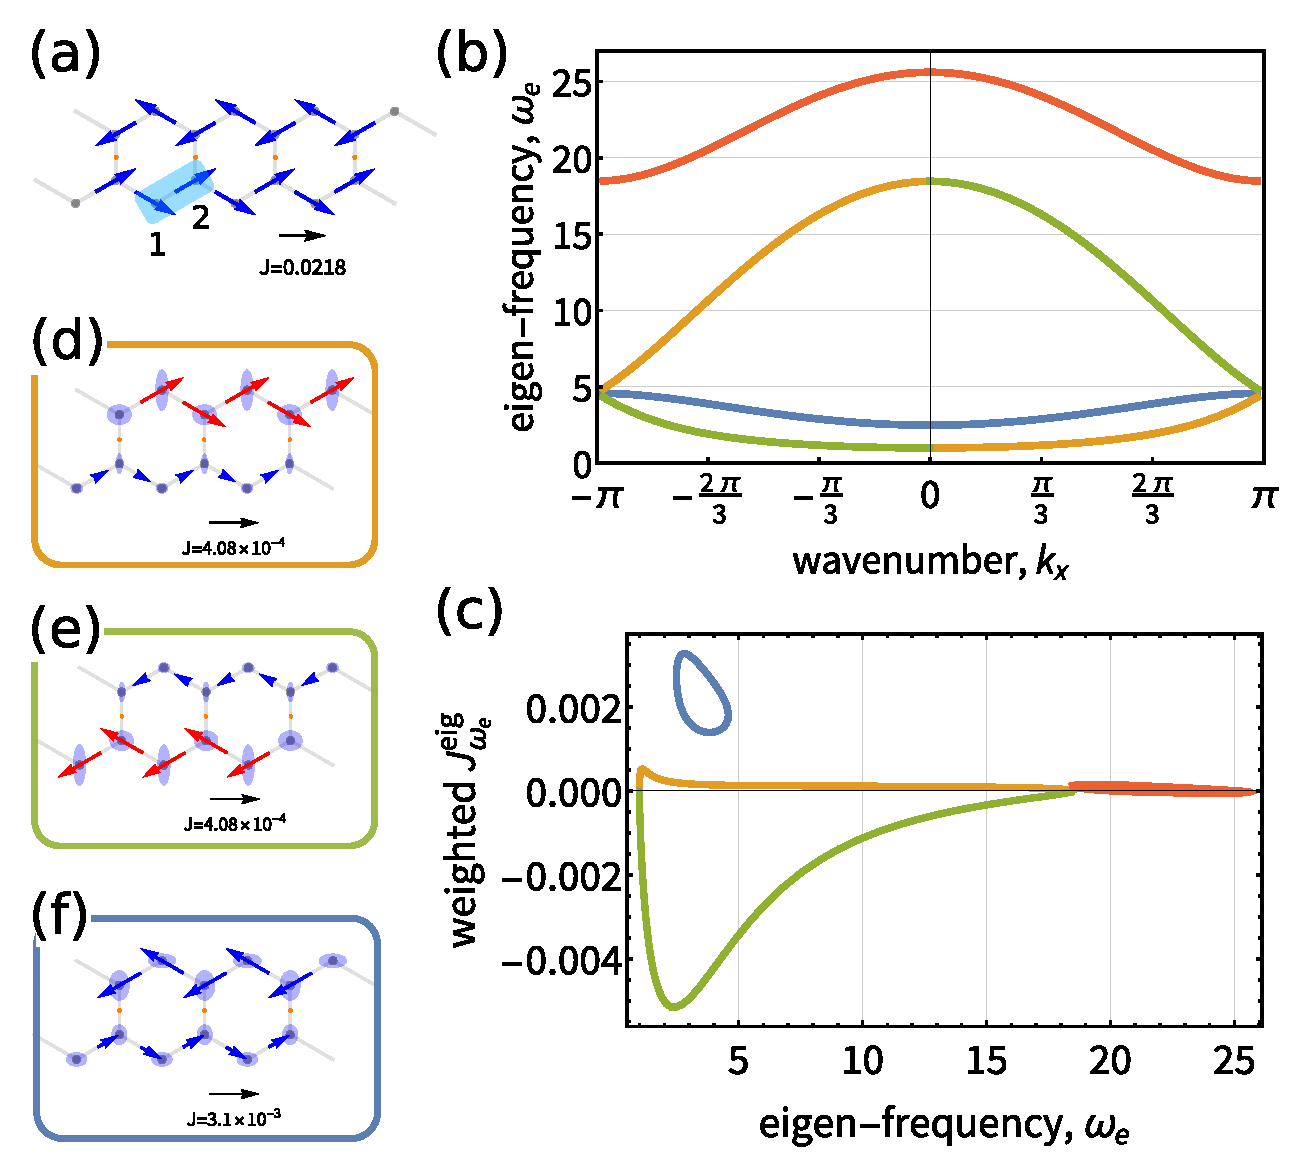
\includegraphics[width=0.45\textwidth]{3_eigen_modes.pdf}
    \caption{Using the eigenmode decomposition, we explain how the flux in honeycomb network is CCW, even though its edgemodes contribute to CW flux.
    (a) Network used for calculation, which consists of one row of hexagons (51 unit cells) and has periodic boundary in $x$ direction. Parameters: $k_{g,\tau}=1, k=10$, others are $1$.
    (b) Band structure of the network (marked with different colors). The yellow/green band contains CW flux localized on the top/bottom edge (an example mode is shown in (d)/(e)). The blue band contains bulk modes with CCW flux (also see (f)).
    (c) Weighted flux $J_{\omega_e}^{eig}$ from $1$ to $2$ (marked in (a)) of the four bands. Total flux in the green band with CW edge modes and the blue band with CCW bulk modes are $-0.106$ and $0.115$, respectively. As a result, the net flux is CCW.
    }
    \label{fig:eigen_modes}
\end{figure}

Since our model is built upon the well-studied isolated system \cite{Nash2015TopologicalMetamaterials,Susstrunk2016ClassificationMetamaterials,Mitchell2018AmorphousSets,Lee2018TopologicalLaws}, we would like to build a connection between our heat flux in the active system and eigenmodes in those studies. We show that the flux formula \eqnname~\eqref{eqn:flux_residue} can be decomposed to a weighted sum over eigenmodes \eqnname~\eqref{eqn:flux_eigen}. Then we apply this result to a honeycomb network as an example.

The Fourier analysis from last section is not suitable for this connection, because Fourier modes and eigenmodes are related only at small $\gamma$'s (\figurename~\ref{fig:Fourier_modes}b and c), but they become dissimilar at larger $\gamma$'s (\figurename~\ref{fig:Fourier_modes}b and d).
The underlying discrepancy between Fourier modes and eigenmodes is that, eigenmodes are for the isolated network, whereas Fourier modes have an extra factor of friction or damping.
In addition to this extra factor $\gamma$, 
the active system also have extra factors of $m$ and $\tau$. The factor $m$ comes from the order of dynamics: the active system is $2$nd order in time, while the gyroscopic dynamics in \cite{Nash2015TopologicalMetamaterials} is $1$st order, which corresponds to the $m\rightarrow 0$ limit.

Our starting equation is \eqnname~\eqref{eqn:flux_residue}. The key bridge for these gaps is that, in $G^+(-i/\tau)$ from the equation, $\gamma,m,\tau$ are not independent factors, they act collectively through $k_{g,\tau} \equiv k_g+\frac{\gamma}{\tau}+\frac{m}{\tau^2}$, so the extra factors $m,\gamma, \tau$ only add a modification to $k_g$. 
We let the reference isolated system we connect to have a modified on-site spring constant $k_{g,\tau}$, then after some algebra, one can show that the flux $\expval{J}$ in active system can be written as a weighted sum of the flux of each eigenmode $J^{\text{eig}}_{\omega_e}$ in the reference system (Supplemental Material),
\begin{equation} \label{eqn:flux_eigen}
\expval{J} = \sum_{\omega_e} \frac{1}{1+\omega_e^2\tau^2} J^{\text{eig}}_{\omega_e}.
\end{equation}
Here $\omega_e$ is the (discrete) eigen-frequency of the reference system, not to be confused with the (continuous) Fourier frequency $\omega$. The amplitude of eigenmode is set such that its energy is $T_a$, and $J^{\text{eig}}_{\omega_e}$ is the time-averaged energy flux.
A related equation is a ``sum rule", the unweighted sum of all modes is zero, $\sum_{\omega_e} J^{\text{eig}}_{\omega_e} = 0$. This can be shown from direct calculation (Supplemental Material).

From this eigenmode decomposition, the discussion of TRS in the isolated system \cite{Nash2015TopologicalMetamaterials} immediately carries over to the active system. For network geometries that satisfy TRS, the energy flux of eigenmodes are zero, thus through \eqnname~\eqref{eqn:flux_eigen}, the flux in active system is also zero. This result can also be obtained from \eqnname~\eqref{eqn:flux_residue}.

As an application, we will analyze the flux in the honeycomb network using the eigenmode decomposition and the ``sum rule".
The flux pattern in the active honeycomb network displays CCW flux localized on the boundary (\figurename~\ref{fig:model_and_result}f). This localization is reminiscent of the edgemode in \cite{Nash2015TopologicalMetamaterials} (\figurename~\ref{fig:Fourier_modes}b), however, their directions are opposite.
From the decomposition \eqnname~\eqref{eqn:flux_eigen}, the edgemodes should contribute a large CW flux in the active system, but somewhat surprisingly, the net flux is CCW.
To better analyze the contribution from each eigenmode {\bf This is a somewhat weird sentence }, we look at a simple honeycomb lattice with only one layer (\figurename~\ref{fig:eigen_modes}a).
This lattice has four bands (\figurename~\ref{fig:eigen_modes}b), two bulk bands (blue, red) and two edge bands (green, yellow). The weighted flux of each band is plotted in \figurename~\ref{fig:eigen_modes}c. We see that the CW edge band does contribute a large CW flux (green curve in \figurename~\ref{fig:eigen_modes}c), however, due to the ``sum rule", the unweighted sum of other bands has to be CCW. In the honeycomb lattice, it happens that many of this CCW fluxes are contained in the lower bulk band (blue curve in \figurename~\ref{fig:eigen_modes}c and example mode in \figurename~\ref{fig:eigen_modes}f). When the flux gets weighted, the CCW flux from lower bulk band outweighs CW flux from the edgemodes, the other two bands (yellow and red curve in \figurename~\ref{fig:eigen_modes}c) also contribute to CCW flux, although relatively small. As a result, the net flux is CCW, which is opposite to the flux of the edgemode.


{\bf A general comment: Since there are a lot of technical things here,I think it will be good to pick and focus on a few (and highlight these at the beginning of sections or subsections). It will be good to explicitly motivate and summarize what the results of each section give us and how they help systematically build towards a particular overarching goal of the paper. That way everything gets tied in and become an excellent narrative. }

\section{Relationship between flux and network geometry} \label{sec:path}
\begin{figure}[ht]
	\centering
	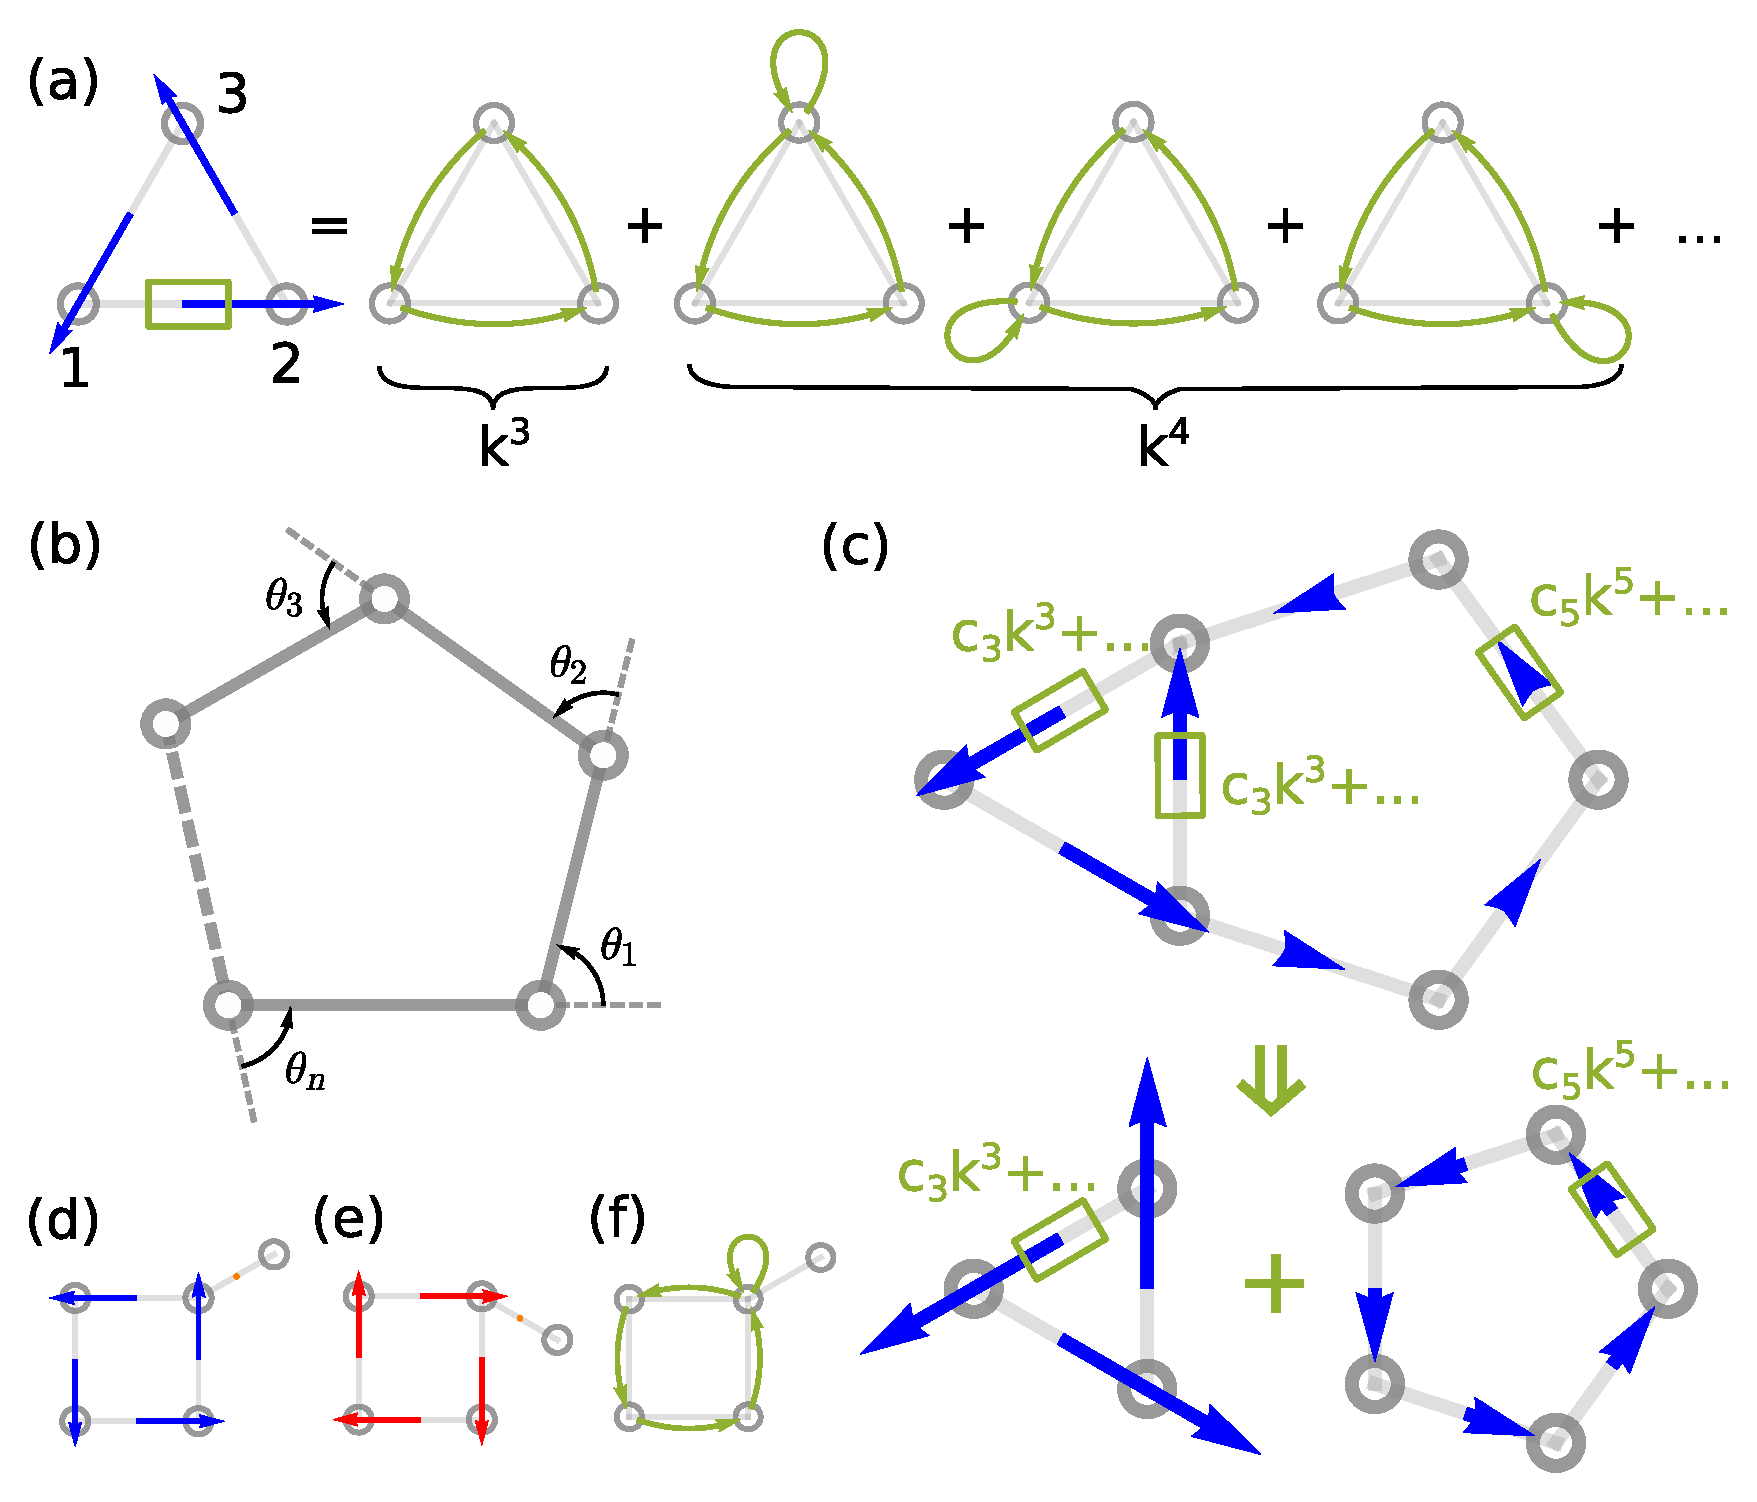
\includegraphics[width=0.45\textwidth]{4_path_sum.pdf}
    \caption{Illustrations of the path summation. 
    (a) Flux from $1$ to $2$ can be calculated by summing over paths. Each path is a diagrammatic representation of one term in the small-$k$ expansion, and is depicted using green arrows. The magnitude of path with length $n$ is on the order of $k^n$. 
    (b) Schematic of a polygon path and its outer angles $\theta_1,\theta_2,\dots,\theta_n$. The flux of this path is simply \eqnname~\eqref{eqn:flux_path_polygon}. 
    (c) For flux in complex networks, the leading order term is determined by the shortest cycles. Flux in the triangle part has order $k^3$, and the pre-factor $c_3$ is the same as that in a standalone triangle network. Likewise for the pentagon part. So the flux in a complex network can be viewed as a result of ``stitching" flux in its cyclic components together.
    (d-f) Direction of flux can be controlled by the orientation of the side-chain. This is because the flux of the lowest-order path (square) vanishes, and the first non-vanishing path (f) is affected by the side-chain.
    }
    \label{fig:path_sum}
\end{figure}

The question on the relationship between the flux and the network geometry can be motivated a few questions based on \figurename~\ref{fig:model_and_result}.
For simple polygon networks, the flux (\figurename~\ref{fig:model_and_result}b-e) should depend on outer angles, does this dependence have an analytic formula?
For more complex networks like the honeycomb in \figurename~\ref{fig:model_and_result}f, its flux pattern seems like a result of combining the flux of single hexagons (\figurename~\ref{fig:model_and_result}c) together. Is there a quantitative description for this speculation?

In this section we explore this relationship using path analysis.
We first expand the flux in small-$k$ regime as a summation over paths in \eqnname~\eqref{eqn:flux_path}, then explain the path rules and diagrammatic representation of the paths.
Since the leading order terms come from the shortest paths, flux analysis is reduced to analyzing only a few paths.
Usual shortest paths are polygonal (without loops), we examine them and answer the two questions above. 
We then also show two examples when higher-order paths with loops are dominant.
Finally, we discuss how this path analysis reveals a simplified dependence on parameters.

{\bf On the whole I like the idea of this paragraph. However, it needs to be rewritten so that the language etc is cleaned up. For instance we should using loose terms like the  ``stiching effect" }

Starting from the flux formula \eqnname~\eqref{eqn:flux_residue}, one can expand the flux to different orders in the spring constant $k$. Then for each order, one can further expand to different paths.
As a result, the total flux can be written as a sum over the flux of paths (\figurename~\ref{fig:path_sum}a), (Supplemental Material)
\begin{equation} \label{eqn:flux_path}
\frac{\expval{J}}{T_a/\tau} = \sum_l J^\text{path}_l = \sum_l \frac{1}{2}(S_l - S_{-l}).
\end{equation}

The path rules are as follows.
For the flux from $i$ to $j$, valid paths are $l=i\rightarrow j\rightarrow l_3\rightarrow l_4\rightarrow \dots \rightarrow l_n\rightarrow i$, where $l_a$ and $l_b$ either has to be bonded or $l_a=l_b$. Paths that contain equal numbers of $i\rightarrow j$ and $j\rightarrow i$ do not contribute (e.g. path $i\rightarrow j\rightarrow i$), because either the path itself vanishes or it cancels with another path. As a result of this, paths appear as cycles.
The term $S_l$ is defined as $S_l \equiv (\frac{k}{k_0})^n \tr R_\alpha (-K_s)_{i l_n} \cdots R_\alpha (-K_s)_{l_3j} R_\alpha (-K_s)_{ji}$,
where $k_0\equiv \sqrt{(k_{g,\tau})^2 + (B/\tau)^2}$ sets the characteristic scale with dimension $k$, $\alpha = \arctan{\frac{B/\tau}{k_{g,\tau}}}$ represents the asymmetry due to $B$-field, $R_\alpha$ is a CCW rotation by angle $\alpha$, and $(K_s)_{l_b l_a} \equiv \frac{1}{k}\bra{l_b}(K-k_gI)\ket{l_a}$ is the geometric factor of spring force on $l_b$ due to the displacement of $l_a$.
$-l$ means $l$ in the reversed order.
The interval of convergence depends on the geometry of the whole network as well as the parameter $\alpha$. The typical value of the upper bound of $\frac{k}{k0}$ ranges between $0.3$ and $0.6$.

The paths can be represented using diagrams, from which the flux $J^\text{path}_l$ can be calculated easily. For instance, the first diagram in \figurename~\ref{fig:path_sum}a represents the path $1\rightarrow 2\rightarrow 3\rightarrow 1$. To calculate $S_l$, one writes $(-K_s)_{l_bl_a}$ for each arrow $l_a\rightarrow l_b$, $R_\alpha$ for each node $l_a$, then multiply these matrices in the reversed order, and calculate the trace. To get $S_{-l}$, one takes the result of $S_l$ and replace $\alpha$ by $-\alpha$. Finally, $J^\text{path}_l$ can be calculated from the difference between $S_l$ and $S_{-l}$.

Path with length $n$ is on the order $(\frac{k}{k_0})^n$, so that in the small $k$ regime, the main contribution to the flux comes from the lowest-order paths. 
The usual lowest-order paths are polygonal cycles with no loops (e.g. $l_a\rightarrow l_a$), in which case, the formula for $J^\text{path}_l$ \eqnname~\eqref{eqn:flux_path} reduces to a simple form (Supplemental Material)
\begin{equation} \label{eqn:flux_path_polygon}
J^\text{path}_\text{polygon} = \frac{1}{2} (\frac{k}{k_0})^n (\prod_i \cos(\theta_i - \alpha) - \prod_i \cos(\theta_i + \alpha)),
\end{equation}
where $n$ is the number of nodes and $\theta_i$'s are outer angles (\figurename~\ref{fig:path_sum}b).
For polygon networks, this formula gives a direct relationship between the lowest-order flux and the network geometry, and all parameters are condensed into a geometric angle $\alpha$. 
For complex networks, this formula quantifies the speculation raised at the section beginning. Since the flux of a polygonal path \eqnname~\eqref{eqn:flux_path_polygon} is not affected by any side chains on the nodes, $J^\text{path}_\text{polygon}$ for a polygon in a complex network is the same as $J^\text{path}_\text{polygon}$ for the polygon when standalone. Therefore the lowest-order flux in a complex network can be viewed as combining the flux of its constituent polygons together. This is illustrated in \figurename~\ref{fig:path_sum}c.

In some situations, the contribution of polygonal paths vanish, and higher order paths with loops become dominant. Unlike in polygonal paths, paths with loops are affected by side-chains.
One situation is when the polygon path itself vanishes. In \figurename~\ref{fig:path_sum}d,e, the flux of lowest order path, square, is zero, so the main contribution comes from the path with length $5$, as shown in \figurename~\ref{fig:path_sum}f. Through the loop in this path, the orientation of the side-chain controls the flux direction in the main square, without changing the geometry of the main cycle (as in \figurename~\ref{fig:model_and_result}c-e).
{\bf It might be good to have a subsection that explains localization due to path summation... the title can be Localization of energy fluxes from path summation .... or something}

Another situation is when two polygon paths cancel each other, which happens in honeycomb-like networks away from the boundary (\figurename~\ref{fig:path_decay}). 
With careful calculations, the fluxes for $n_l\ge 1$ are not zero, they rather appear as an exponential decay (\figurename~\ref{fig:path_decay}b). By changing the network geometry $\theta$, the decay length varies non-monotonically, and has a cusp at $\theta=\alpha$ (\figurename~\ref{fig:path_decay}c). 
This decay and its relationship with $\theta$ can be explained by considering the paths.
While the polygon path constitutes the lowest-order path at the boundary (\figurename~\ref{fig:path_decay}d), it vanishes for $n_l\ge 1$ due to cancellations (\figurename~\ref{fig:path_decay}e). The first non-vanishing pair of paths for $n_l=1$ is shown in \figurename~\ref{fig:path_decay}f, in which the loop exploits the asymmetry between the bulk side (has a vertical bond at the blue loop) and the boundary side (has no vertical bonds at the red loop). For every increment of one layer, the length of paths increases by $4$ (\figurename~\ref{fig:path_decay}g,h). So the flux at layer $n_l$ is on the order of $k^{4n_l+3}$, which exhibits an exponential decay $e^{-(n_l-1)/d_l}$. 
Through the calculation of these paths, one gets the decay length $d_l = -1/\log[4(k/k_0)^4(\sin(\theta+\alpha)\sin(\theta-\alpha))^2]$. From this result, we see that the cusp at $\theta=\alpha$ in \figurename~\ref{fig:path_decay}c is due to the term $\sin(\theta-\alpha)$. In fact, at the special point $\theta=\alpha$, paths in \figurename~\ref{fig:path_decay}f-h vanish, and one needs to consider even high-order paths.

\begin{figure}[ht]
	\centering
	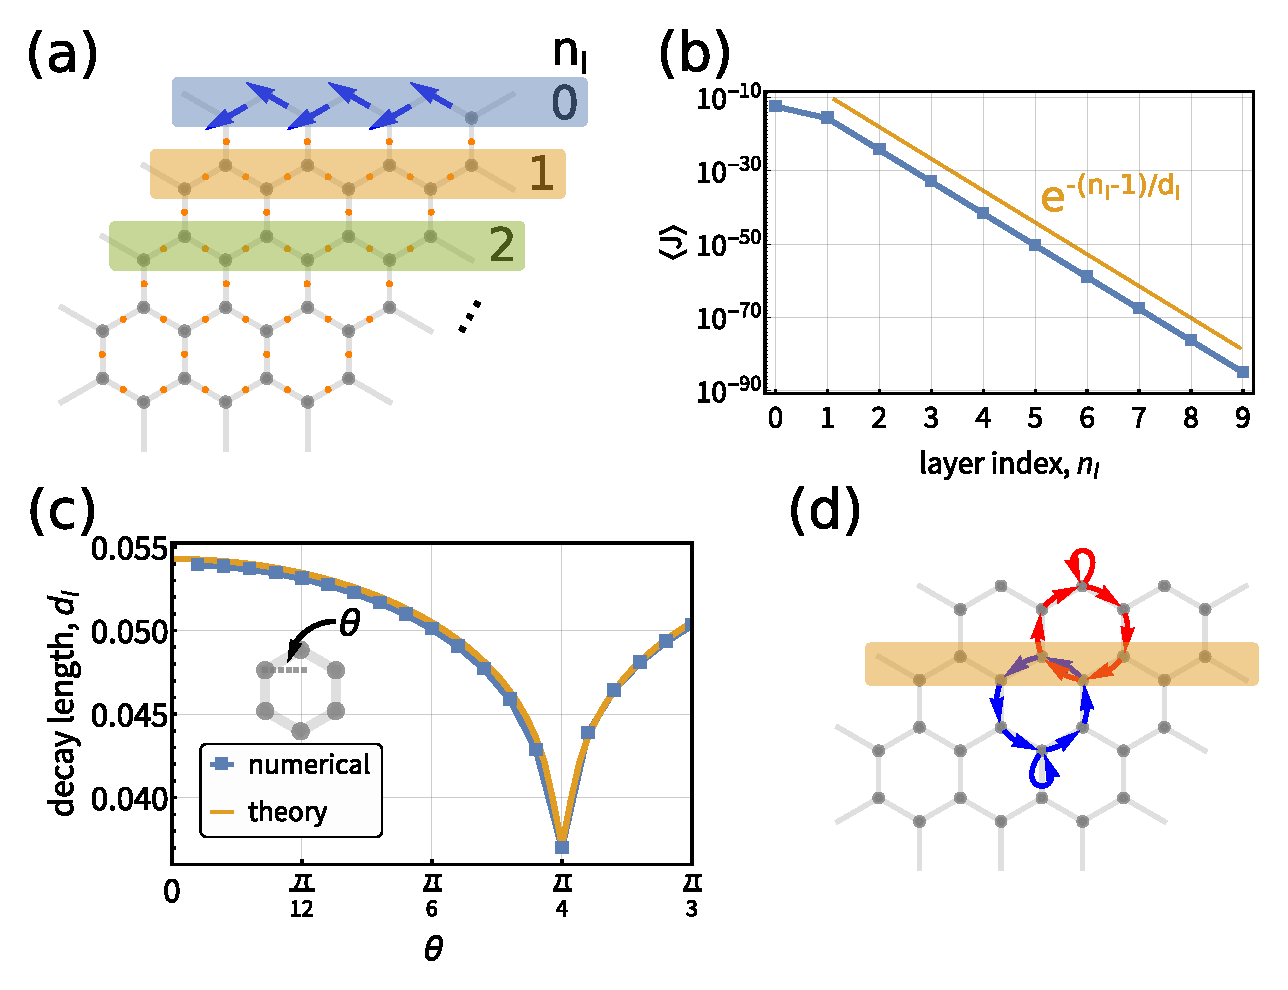
\includegraphics[width=0.45\textwidth]{5_path_decay.pdf}
    \caption{Decay of fluxes away from the boundary of honeycomb networks, and explanation using the path picture.
    (a) Schematic of a honeycomb network which is periodic in the $x$ direction. Layers from the boundary are indexed as $n_l$.
    (b) Semi-log plot of flux $\expval{J}$ at layer $n_l$. The flux starting from layer $n_l=1$ shows exponential decay, with decay length $d_l$. Parameters: $\theta = \pi/6, k/k_0 = 0.01, \alpha = \pi/4$.
    (c) Decay length $d_l$ changes with the network angle $\theta$ non-monotonically, and the curve has a cusp at $\theta = \alpha = \pi/4$. At small $k/k_0$, perturbation theory results agree with numerical calculations.
    (d) The lowest-order flux of $n_l=0$ comes from the hexagon path ($\expval{J}\sim k^6$).
    (e) For $n_l=1$, a pair of $k^6$ paths (blue and red) cancel each other. 
    (f) The first non-vanishing path pair for $n_l=1$ has length $7$. The two paths do not cancel, because the loop in the bulk and at the boundary have different values.
    (g,h) Two examples of non-vanishing pairs for $n_l=2$. Their length is $11$.
    }
    \label{fig:path_decay}
\end{figure}

At the end of this section, we discuss the dependence of flux on parameters. 
For a fixed network geometry, originally the flux is affected by $7$ parameters, however, \eqnname~\eqref{eqn:flux_path_polygon} tells us that these parameters can be condensed to one parameter $\alpha$. 
How this reduction of parameters happens is summarized as follows. 
Originally, the flux $\expval{J}$ is a function of all the parameters, $\expval{J} = f(m, k_g, k, B, \gamma, \tau, T_a)$.
From the linear response theory, we found that $k_g, \gamma, m$ affects the flux as a combination $k_{g,\tau} \equiv k_g + \frac{\gamma}{\tau} + \frac{m}{\tau^2}$, and $B$ appears as $B_\tau \equiv \frac{B}{\tau}$. So the parameters are reduced to $\frac{\expval{J}}{T_a/\tau} = f(k_{g,\tau}, k, B_\tau)$.
The parameters on the right hand side can be further non-dimensionalized by  $k_0$, to give $\frac{\expval{J}}{T_a/\tau} = f(\frac{k}{k_0}, \alpha)$.
In the small-$k$ expansion, the ratio $\frac{k}{k_0}$ can be taken out, so the flux is just a function of $\alpha$, $\frac{\expval{J}}{T_a/\tau} = f(\alpha) (\frac{k}{k_0})^n + \order{(\frac{k}{k_0})^{n+1}}$, where $n$ is the length of the shortest path.


\section{A sample trajectory from simulation} \label{sec:simulation}
{\bf what is the purpose of this section ? Why can't it be in the SI ? }
\begin{figure}[ht]
	\centering
	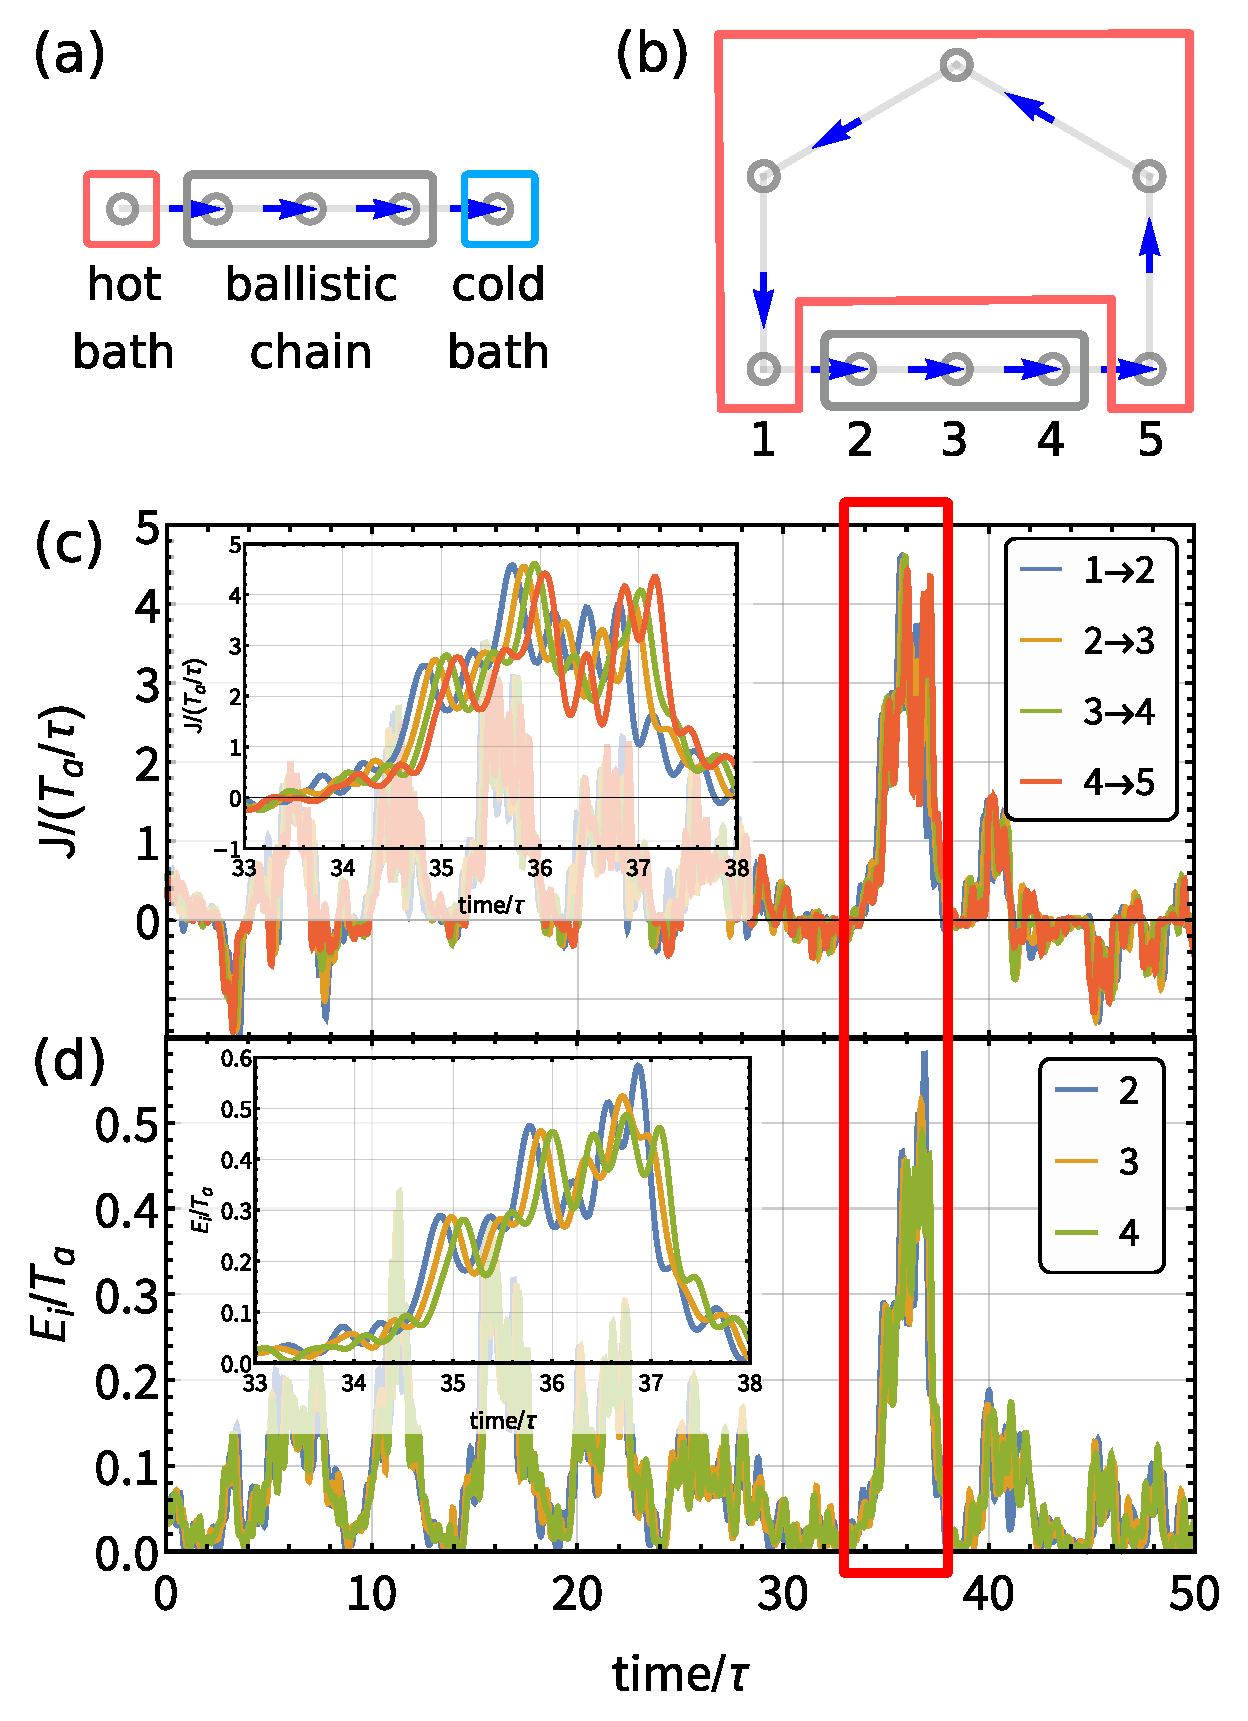
\includegraphics[width=0.45\textwidth]{6_simulation.pdf}
    \caption{Flux in a sample trajectory.
    (a) Conventional heat conduction in a chain with temperature differences at two ends. The temperature difference drives a heat flow through the ballistic chain.
    (b) Similar to (a), the active gyroscopic network can also drive a heat flow through a ballistic segment. In the simulation setup, the separation between active particles (boxed in red) is large compared with the length-scale of their displacements, and their parameters are: $m,k_g,\gamma=0.1, k=10$, others are $1$. Ballistic particles (boxed in gray) are restrained to 1D, and their $\gamma,T_a,k_g$ are set to $0$.
    (c) Flux $J$ through bonds in the ballistic part in the trajectory. $J$ is random in general, however, during the period when $J$ is large, as the example boxed in red, $J$ shows (see the inset) successive peaks in accordance with the direction of the flux.
    (d) Energy of each particle in the ballistic part shows similar features to the flux. In particular, it also shows successive peaks.
    }
    \label{fig:simulation}
\end{figure}

Using computer simulations, we show some features of the (instantaneous) heat flux in the time domain.
Simulations are performed using LAMMPS \cite{Plimpton1995FastDynamics} with the tool Moltemplate \cite{Jewett2013MoltemplateTool} and custom code (Supplemental Material).
In the conventional heat conduction, temperature difference at the boundary can drive the heat flow through a ballistic segment (\figurename~\ref{fig:simulation}a). Using an analogous setup, we add a ballistic segment to the active network (\figurename~\ref{fig:simulation}b). In this segment, we set $\gamma,T_a,B,k_g=0$, so there is no direct influence from the active bath or the $B$-field.
Numerical calculation (\figurename~\ref{fig:simulation}b) shows that there is heat flow passing through the ballistic segment. From the view of this segment, the active part acts like a ``battery", similar to the conventional case (\figurename~\ref{fig:simulation}a).
From computer simulations (\figurename~\ref{fig:simulation}c,d), the flux through bonds in the ballistic segment is in general random. During the period when $J$ is large, $J$ shows successive peaks, indicating a large energy flow from left to right. The spacing between the peaks matches the sound speed of the ballistic chain ($\sqrt{k/m}$). Although the direction of flux is from left to right on average, the instantaneous flux can also transport from right to left, shown as negative peaks in \figurename~\ref{fig:simulation}c. Similar features also present in the energy of each particle (\figurename~\ref{fig:simulation}d).


\section{Implications for swimmer and fluid pumping} \label{sec:swimmer}

\begin{figure}[ht]
	\centering
	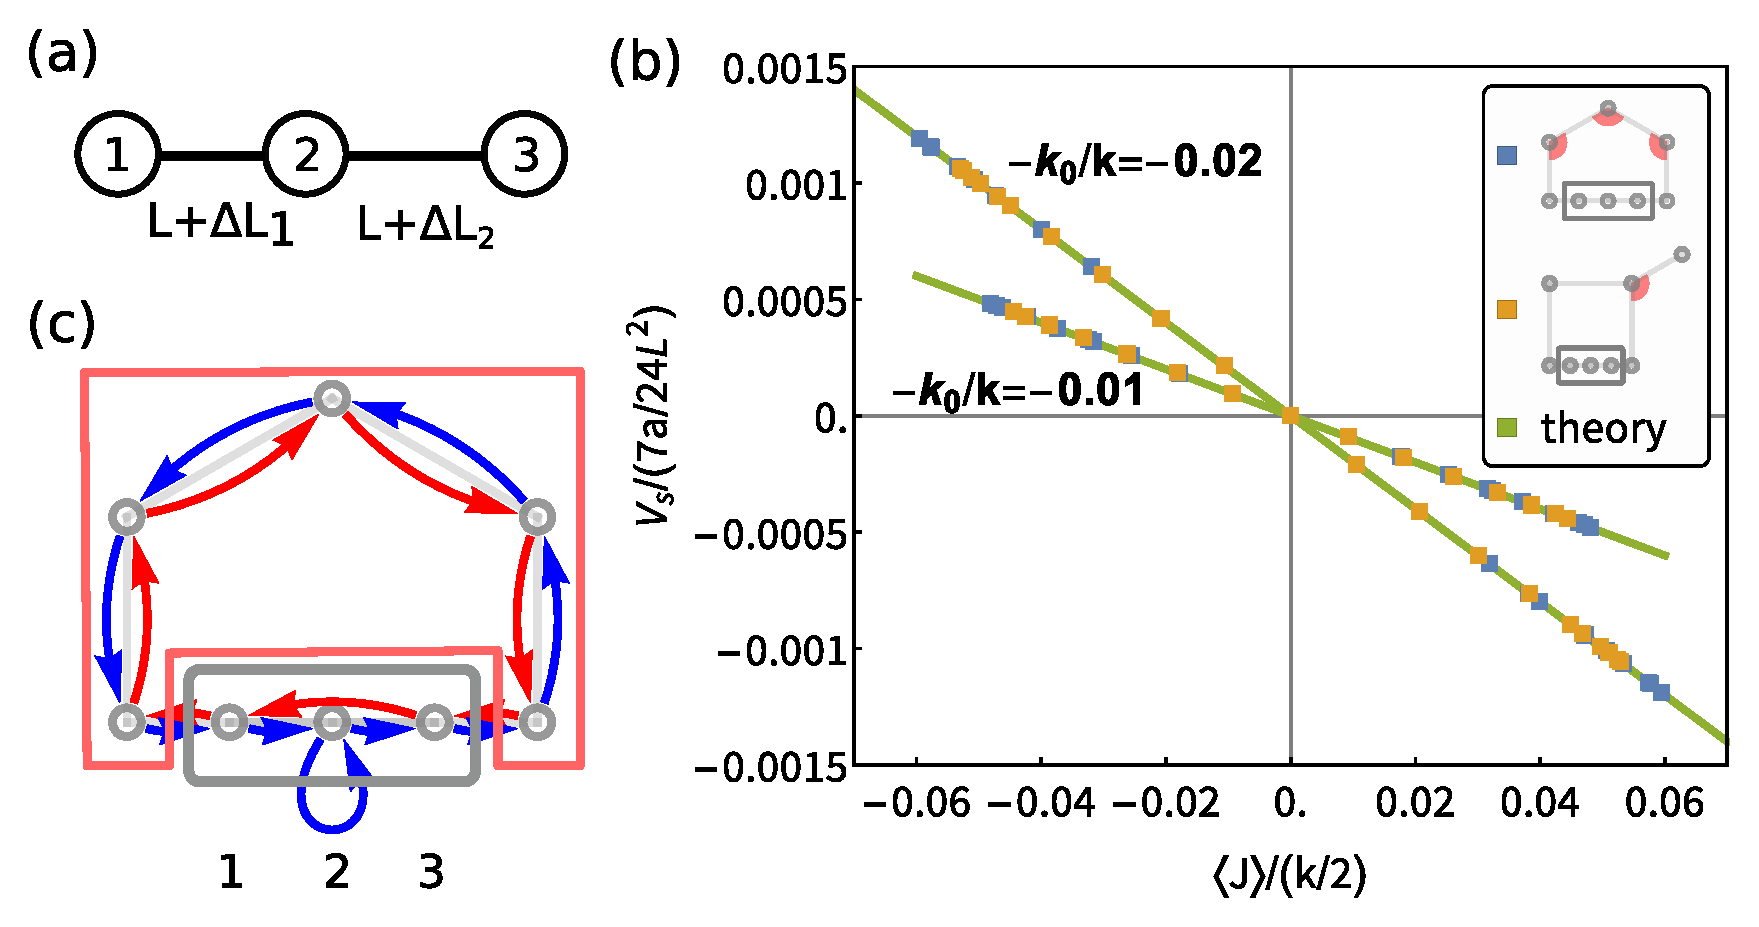
\includegraphics[width=0.45\textwidth]{7_swimmer.pdf}
    \caption{Active network dynamics as a swimming protocol.
    (a) Three-sphere swimmer model from \cite{Golestanian2008AnalyticNumber}. In order to swim, the swimmer vary the lengths of its two legs according to some protocol.
    (b) Swimmer's speed $V_s$ is directly proportional to the energy flux $\expval{J}$ in the active network. The proportionality constant is $-k_0/k$, which is independent of the network geometry. The series of dots for each $-k_0/k$ are obtained by varying the labelled angles (by red disk sectors) in pentagon networks or square+tail networks.
    (c) One example of $J_{31}^s$ path (red) and $J_{12}^s$ path (blue). Ballistic particles are boxed in gray, and the active ones are boxed in red.
    }
    \label{fig:swimmer}
\end{figure}

The energy flux has been our main focus so far. At last we discuss its further implications in a different context of swimmers at low Reynolds numbers ($Re$).
One similarity between low-$Re$ swimmers and active networks is that, swimmers' motion has to be non-reciprocal or TRS-breaking in order to swim, and the energy flux in active networks also indicates TRS-breaking motions.
We first show that, if a three-sphere swimmer \cite{Golestanian2008AnalyticNumber} (\figurename~\ref{fig:swimmer}a) uses a swimming protocol according to the dynamics of ballistic particles in \figurename~\ref{fig:simulation}b, it can swim, and the swimming speed is directly proportional to the energy flux (\eqnname~\eqref{eqn:swimmer_propto}).
Based on this result, we then discuss the possibility of generating fluid flows if we immerse the ballistic particles into a fluid and make them a swimmer.

In Ref.\cite{Golestanian2008AnalyticNumber}'s setup, a linear three-sphere swimmer as \figurename~\ref{fig:swimmer}a is immersed in a low $Re$ fluid. When the swimmer changes the lengths of its two legs according to some protocol, which is described by a constant part $L$ plus a varying part $\Delta L_i$ for $i=1,2$, the time-averaged swimming speed is (\eqnname~(12) in \cite{Golestanian2008AnalyticNumber})
\begin{equation} \label{eqn:swimmer_speed}
    V_s = \frac{7a}{24L^2} \expval{\Delta L_1 \Delta \Dot{L_2} - \Delta \Dot{L_1} \Delta{L_2}},
\end{equation}
where $a$ is the radius of the swimmer. Assumptions for this equation are $a/L \ll 1, \Delta L_i/L \ll 1$, and external force on the swimmer is zero.

We set the swimming protocol to be the motions of the three ballistic particles in active networks like \figurename~\ref{fig:simulation}b (except that here we allow $k_g$ of ballistic particles to be nonzero),
and compute $V_s$ of the swimmer and compare it with the energy flux $\expval{J}$ from the active network. 
The $V_s-\expval{J}$ plot in \figurename~\ref{fig:swimmer}b shows that, the swimmer using our protocol can swim, and the speed $V_s$ is proportional to $\expval{J}$. Moreover, this proportionality constant does not depend on the network geometry. 
In fact, this constant can be calculated using a modified path analysis (Supplementary Material), 
\begin{equation} \label{eqn:swimmer_propto}
    \frac{V_s}{7a/24L^2} = -\frac{k_0}{k} \frac{\expval{J}}{k/2},
\end{equation}
where $k_0 = k_g + m/\tau^2$ ($B,\gamma=0$ for the ballistic part).
This result \eqnname~\eqref{eqn:swimmer_propto} holds beyond small-$k$ regime because all paths are considered (\figurename~\ref{fig:swimmer}c, and Supplementary Material).
Both \figurename~\ref{fig:swimmer}b and \eqnname~\eqref{eqn:swimmer_propto}  establish that one can dictate swimmer's speed from the energy flux of active networks.

Now consider a different but related scenario, where we immerse the ballistic segment in a fluid. Since the segment is tethered by $k_g$ and is connected to the tethered active part, it cannot swim indefinitely. But will it pump the fluid instead?
To answer this question, we need to discuss three issues with translating result \eqnname~\eqref{eqn:swimmer_propto} to this scenario.

Firstly, due to additional forces from tethering, \eqnname~\eqref{eqn:swimmer_speed} for $V_s$ does not directly apply, and modifications are needed.
Ref. \cite{Golestanian2008AnalyticNumber} discussed swimmer with a constant external force $F$, and its \eqnname~(39) says the modified swimming speed $V_s(F) = V_s + F/(6\pi\eta a)$. Since this result is obtained under linearized hydrodynamics, it also applies to our stochastic case if we replace $F$ by its averaged value $\expval{F}$.

Secondly, the added fluid should not alter the original dynamics too much, otherwise both the energy flux and the correlation in \eqnname~\eqref{eqn:swimmer_speed} would be distorted, and one cannot utilize the $V_s \propto -\expval{J}$ result. Can we treat the fluid as a perturbation? To make the hydrodynamic interactions perturbative, one can set $a/L \ll 1$. To make the Stokes drag coefficient $\gamma_s \equiv 6\pi\eta a$ perturbative, where $\eta$ is fluid's dynamic viscosity, one can set $a \ll 1, \eta \sim 1$ (with proper dimensions). This setup can satisfy the low $Re$ condition $\rho v a/\eta \ll 1$ by letting $\rho,v \sim 1$, where $\rho$ is the fluid density, and satisfy the overdamped dynamics (with no fluctuations) by letting $m \ll \gamma_s$. 
These settings are self-consistent. With these settings, one can approximate the particles' dynamics in a fluid by their original dynamics, and the error is on the order of $\gamma_s a / L$.

Lastly, what does a stalled swimmer do to the fluid? From an experimental study \cite{Leoni2009ANumber}, we know that the stalled swimmer can generate a fluid flow in the opposite direction.

These discussions together suggest that, if the ballistic part is immersed in a perturbative fluid, it can generate fluid flows.
Assuming the relaxation timescale of the active network is much faster than the timescale of swimming due to the small $V_s(F)$, one can expect the following process. Initially the ballistic part experiences $\expval{F}=0$, so it swims with speed $V_s$; as the part drifts, $\expval{F}$ increases and acts in the direction of $-V_s$; when $\expval{F} \approx -6\pi\eta a V_s$, the swimmer is stalled. The stalled swimmer pumps fluid in direction $-V_s \propto \expval{J}$.


\section{Conclusion} \label{sec:conclusion}

In previous discussions, the parameters are assumed uniform for all particles and bonds, which is not necessary.
The Fourier mode and path summation analyses only needs $\tau,T$ to be uniform. The eigenmode decomposition further needs $B$ to be uniform and non-vanishing.

If we add an additional white noise to the equation of motion \eqnname~\eqref{eqn:GLE_single}, the flux is not affected. As a comparison, in models that use OUP for directed particle transport, the additional white noise would usually suppress the rectification \cite{Bartussek1996PreciseRatchets}.

By combining the gyroscopic network and the active bath, one can generate unconventional heat flows. 
From Fourier decomposition, eigenmode decomposition, and path summation, respectively, we understand the mechanism of this nonzero heat flow, the connection between the flow in active system and that in the well-studied isolated system, and the relationship between the network geometry and the flow pattern.
In particular, the path perspective reveals that, this stochastic system has some simple statistical properties that do not need the knowledge of the underlying modes. Using this perspective, one can in turn achieve controlling the flux pattern by the design of network geometries.


\section*{Acknowledgements}
We thank many people.


\bibliography{reference}

\end{document}
